Les systèmes physiques composés de nombreuses particules identiques se comportent très différemment en fonction des échelles de distance et de temps auxquelles ils sont sondés. Dans un gaz très dilué, sur des échelles de temps pas plus grandes que le temps typique entre deux collisions, les particules sont essentiellement non-interactives. Ainsi, deux nuages de fluide peuvent entrer en collision et simplement se traverser ; un exemple familier de ce phénomène en astrophysique est celui des nuages d'étoiles dans les galaxies en collision. En revanche, sur des échelles de temps beaucoup plus longues que le temps de collision, les particules subissent généralement un très grand nombre de collisions, de sorte que le fluide a le temps de se relaxer localement vers un état d'équilibre. Cette relaxation locale donne lieu à un comportement hydrodynamique, qui est typiquement bien plus complexe et non-linéaire que la simple propagation libre. Par exemple, on peut penser à deux gouttes d'eau qui entrent en collision : elles ne vont pas simplement se traverser. Il est plus probable que leur mouvement soit plus complexe, par exemple qu'elles se coalescent~\citep{brazier1972interaction}.


\vspace{0.5cm}




La dynamique des fluides à courts temps est capturée par une équation d'évolution pour la densité dans l'espace des phases des particules $\rho(x,p,t)$ qui prend la forme d'une équation de transport libre, ou équation de Boltzmann sans collision. Typiquement,
\begin{equation}
	\label{eq:liouville}
	\frac{\partial}{\partial t} \rho(x,p,t)  + v(p)  \frac{\partial}{\partial x} \rho(x,p,t) -   \frac{\partial  V(x)}{\partial x}  \frac{\partial}{\partial p} \rho(x,p,t)   \, = \, 0.
\end{equation}
Ici, nous écrivons l'équation dans une dimension spatiale ; l'extension aux dimensions supérieures est directe. Dans l'équation (\ref{eq:liouville}), $v(p)$ est généralement la vitesse de groupe $ \partial \varepsilon(p)/\partial p$ d'une particule ayant un moment $p$ et une énergie cinétique $\varepsilon(p)$, et $V(x)$ est un potentiel externe. L'équation~(\ref{eq:liouville}) est obtenue, par exemple, pour $N$ particules classiques décrites par le Hamiltonien non-interactif $\mathcal{H} = \sum_{j=1}^N [ \varepsilon(p_j) + V(x_j) ]$. L'évolution de la densité dans l'espace des phases $\rho(x,p,t) = \sum_{j=1}^N  \delta(x - x_j(t) ) \delta(p-p_j(t))$ découle alors de l'évaluation du crochet de Poisson $\partial \rho / \partial t = \{ \mathcal{H}, \rho  \}$. Des équations similaires à l'équation~(\ref{eq:liouville}) apparaissent dans la description de fluides constitués de particules à la fois classiques et quantiques ; nous y reviendrons ci-dessous.

 
\vspace{0.5cm}


Sur des échelles de temps bien plus longues que le temps de relaxation, l'équation~(\ref{eq:liouville}) est supplantée par un système d'équations hydrodynamiques. À cette échelle, le fluide est localement relaxé vers un état d'équilibre à tout moment. Les états d'équilibre local sont paramétrés par les quantités conservées du système, dont l'évolution dans le temps est régie par des équations de continuité. Un bon exemple est celui d'un fluide galiléen avec un nombre de particules conservé, un moment conservé et une énergie conservée. Une description hydrodynamique moyennée, valide à grande échelle de distance et de temps, est obtenue en écrivant trois équations de continuité pour la densité de masse $q_M$, la densité de moment $q_P$, et la densité d'énergie $q_E$,
\begin{equation}
	\label{eq:continuity3}
	\left\{  \begin{array}{ccc}
		\frac{\partial}{\partial t} q_M (x,t)+ \frac{\partial}{\partial x}   j_{M} (x,t)  &=& 0 \\ 
		\frac{\partial}{\partial t}  q_P (x,t) + \frac{\partial}{\partial x}  j_{P} (x,t) &=& - \frac{1}{m}  \frac{\partial V(x)}{\partial x} q_M (x,t )  \\ 
		\frac{\partial}{\partial t}  q_E (x,t) +\frac{\partial}{\partial x}  j_{E} (x,t)   &=& 0  ,
	\end{array} \right.
\end{equation}
où $j_M$, $j_P$ et $j_E$ sont les trois courants associés. Ici, la deuxième ligne n'est pas tout à fait une équation de continuité, sauf si $\partial V/\partial x = 0$. Cela est simplement dû au fait que le moment n'est pas conservé en présence d'une force externe : le membre de droite de cette équation d'évolution pour $q_P$ est donné par la deuxième loi de Newton.

En raison de la relaxation locale, les courants dépendent de $x$ et $t$ uniquement à travers leur dépendance aux densités de charge. En général, un courant $j$ est une fonction de toutes les densités de charge $q$ et de leurs dérivées spatiales $\partial_x q$, $\partial_x^2 q$, etc. Cependant, pour des variations de densité de très longues longueurs d'onde, la dépendance aux dérivées peut être négligée, et 
$j_M$, $j_P$ et $j_E$ sont des fonctions de $q_M$, $q_P$ et $q_E$ uniquement. Les équations hydrodynamiques d'ordre zéro obtenues de cette manière sont généralement appelées `hydrodynamique à l'échelle d'Euler' ou `limite hydrodynamique d'Euler'. À l'échelle d'Euler, les trois équations de continuité ci-dessus se réduisent aux équations d'Euler standards pour un fluide galiléen,
\begin{equation}
	\label{eq:euler}
	\left\{  \begin{array}{ccc}
		\frac{\partial}{\partial t} n + \frac{\partial}{\partial x}  (nu) &=& 0 \\ 
		\frac{\partial}{\partial t} u + u \frac{\partial}{\partial x} u + \frac{1}{m n} \partial_x \mathcal{P} &=& - \frac{1}{m} \frac{\partial V}{\partial x}   \\ 
		\frac{\partial}{\partial t}  e + u \frac{\partial}{\partial x}  e + \frac{1}{n} \mathcal{P} \partial_x u  &=& 0  .
	\end{array} \right.
\end{equation}
Ici, $m$ est la masse des particules, $n = q_M/m$ est la densité de particules, $u = q_P/q_M$ est la vitesse moyenne du fluide, et $e = (q_E - q_P^2/(2 q_M) - n V(x) ) /n$ est l'énergie interne par particule. Pour passer des équations de conservation~(\ref{eq:continuity3}) au système~(\ref{eq:euler}), on utilise le fait que $j_M = q_P$ en raison de l'invariance galiléenne. De plus, à l'échelle d'Euler, $j_P = q_P^2/q_M + \mathcal{P}$ et $j_E =  (q_E + \mathcal{P}) q_P/q_M$, où $\mathcal{P} = \mathcal{P}(n,e)$ est la pression à l'équilibre.

Pour fermer le système d'équations~(\ref{eq:euler}), il faut connaître la pression à l'équilibre $\mathcal{P}(n,e)$, qui est une fonction de $n$ et $e$ et qui dépend des détails microscopiques du système. Dans certains modèles simples tels que le gaz parfait, une expression analytique simple pour la pression est disponible, mais en général il n'y en a pas. Pour le gaz de Bose unidimensionnel avec répulsion de contact, qui est au centre de cet article de revue, $\mathcal{P}(n,e)$ peut être tabulée numériquement (voir la sous-section \ref{subsec:yangyang}).

Pour conclure cette brève discussion des équations hydrodynamiques, mentionnons qu'il est bien sûr possible d'aller `au-delà de l'échelle d'Euler', et de faire de l'hydrodynamique du premier ordre en conservant la dépendance des courants aux gradients des densités de charge. Cela conduit à des équations hydrodynamiques de type Navier-Stokes, qui incluent

 des termes dissipatifs. Dans cet article de revue, nous nous concentrons principalement sur l'hydrodynamique à l'échelle d'Euler (ordre zéro).
 
 \vspace{0.5cm}

Cet article de revue traite du comportement particulier semblable à un fluide qui émerge dans le gaz de Bose unidimensionnel quantique. Il est particulier en ce sens qu'il est simultanément sous la forme (\ref{eq:continuity3},\ref{eq:euler}) et sous la forme (\ref{eq:liouville}), sur des échelles de temps beaucoup plus longues que l'inverse du taux de collision. Ce même comportement particulier est commun à tous les systèmes intégrables unidimensionnels, qu'ils soient classiques ou quantiques, et il est connu sous le nom d'Hydrodynamique Généralisée' ou GHD' depuis 2016~\citep{castro2016emergent,bertini2016transport}. Ici, le terme Généralisée' est utilisé de la même manière que dans Ensemble Gibbs généralisé' \citep{rigol2007relaxation,rigol2008thermalization} : il désigne l'extension d'un concept (Ensemble de Gibbs' ou Hydrodynamique') du cas avec un petit nombre fini de quantités conservées au cas avec une infinité de celles-ci.

\vspace{0.5cm}

Pour illustrer l'émergence de l'Hydrodynamique Généralisée' dans un système avec une infinité de quantités conservées, il est instructif de penser à \(N\) billes de billard identiques de diamètre \(|\Delta|\) dont le mouvement est restreint à une ligne unidimensionnelle, voir Fig.~\ref{fig:hardrod}. Ici, nous prenons \(\Delta < 0\). [Cette drôle de convention garantit que les équations hydrodynamiques pour le gaz de hard core (\ref{eq:GHDintro}) sont presque les mêmes que celles pour le gaz de Lieb-Liniger, voir Eq.~(\ref{eq:ghd}). \(\Delta\) est positif dans le gaz de Bose unidimensionnel répulsif, voir la Sous-section~\ref{subsec:Wigner}.] Ce modèle pour un gaz unidimensionnel classique est connu sous le nom de gaz de hard rod' dans la littérature de la physique statistique, voir e.g.~\citep{percus1976equilibrium,lebowitz1967kinetic,aizenman1975ergodic,boldrighini1983one,spohn2012large,boldrighini1997one,doyon2017dynamics,cao2018incomplete}. Les billes sont à la position \(x_j\) et se déplacent à la vitesse \(v_j\), \(j=1,\dots , N\). Lorsque deux billes entrent en collision de manière élastique, elles échangent leurs vitesses, si bien que l'ensemble des vitesses est conservé à tout moment. Ainsi, ce système de plusieurs particules a une infinité de quantités conservées qui sont indépendantes dans la limite thermodynamique \(N\rightarrow \infty\). En effet, pour toute fonction \(f\) de la vitesse, la charge \(Q[f] := \sum_{j=1}^N f(v_j)\) est conservée.

\begin{figure}[ht]
    \centering
    \begin{tikzpicture}
    \draw (0,0.4) node{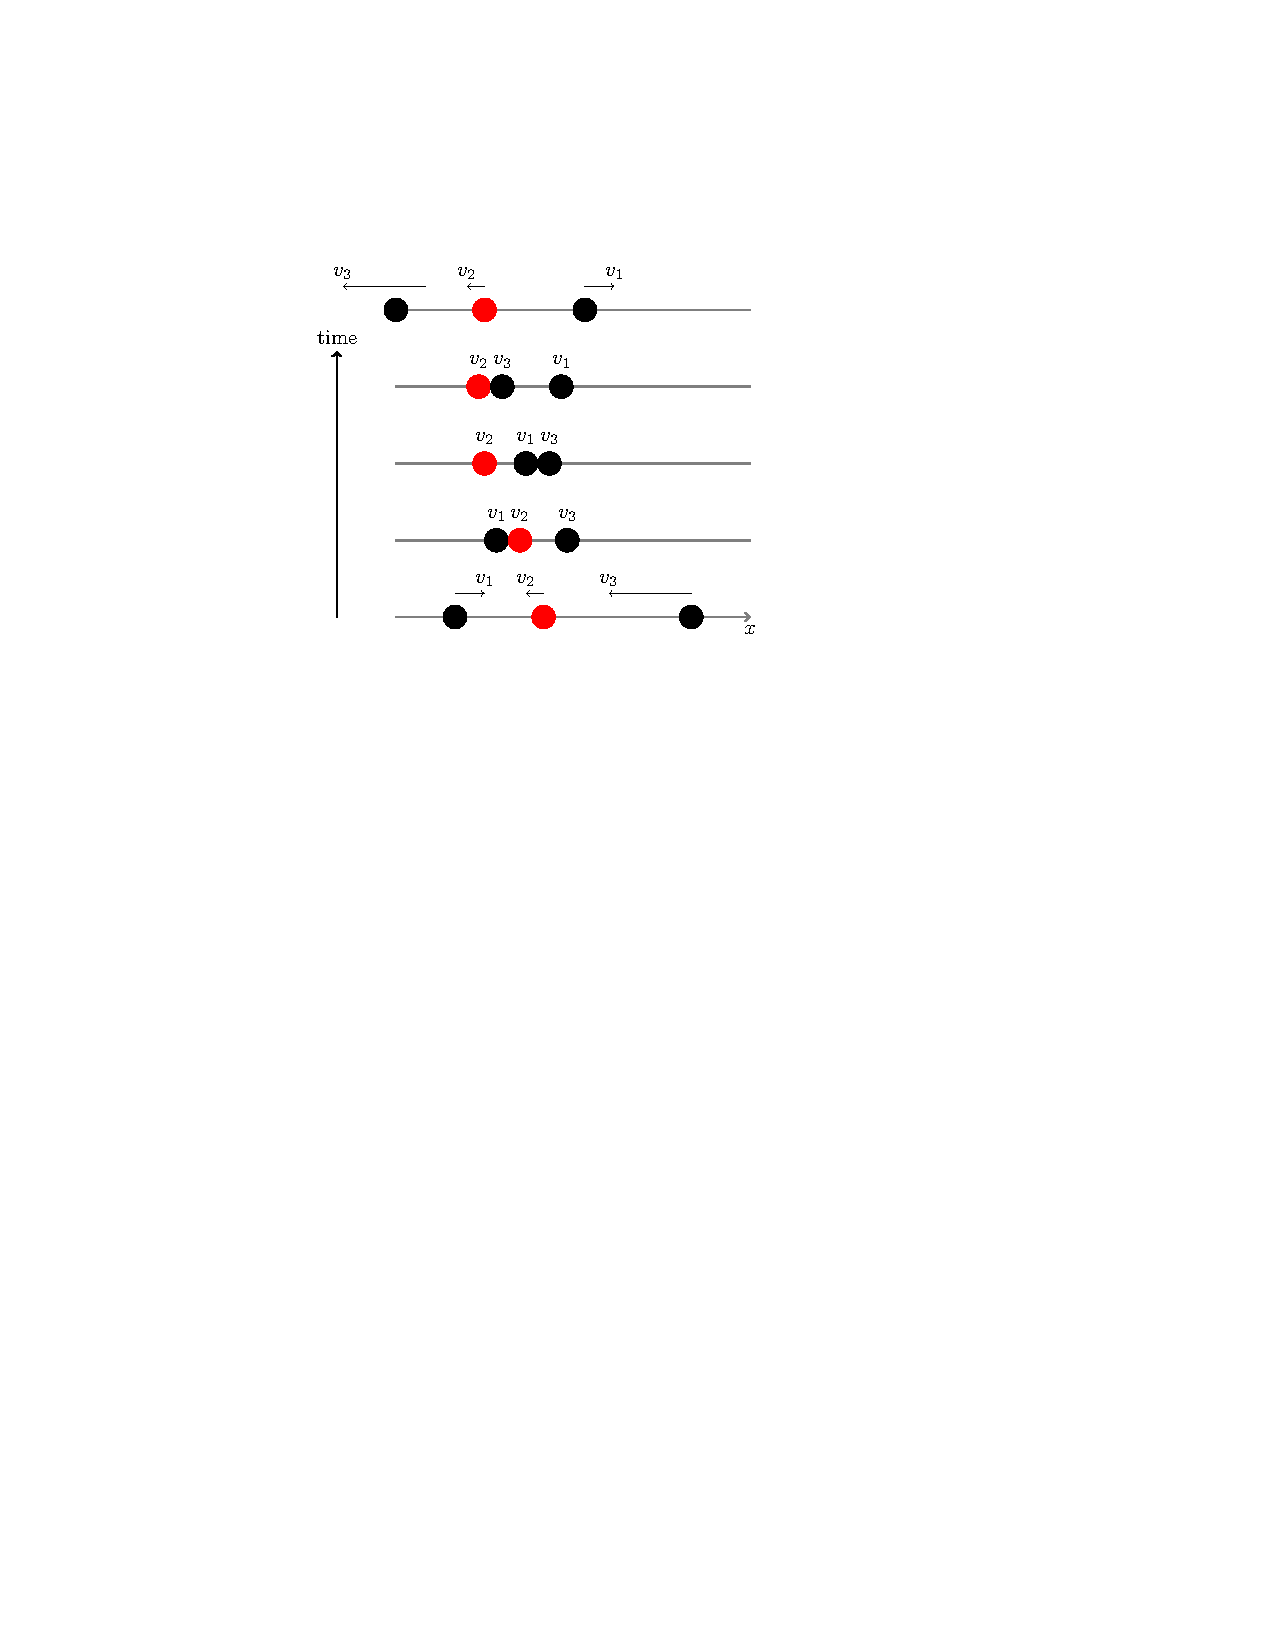
\includegraphics[width=0.35\textwidth]{doc/arXiv-2108.02509v2/figures/hardrods2.pdf}};
    \draw (7.7,0) node{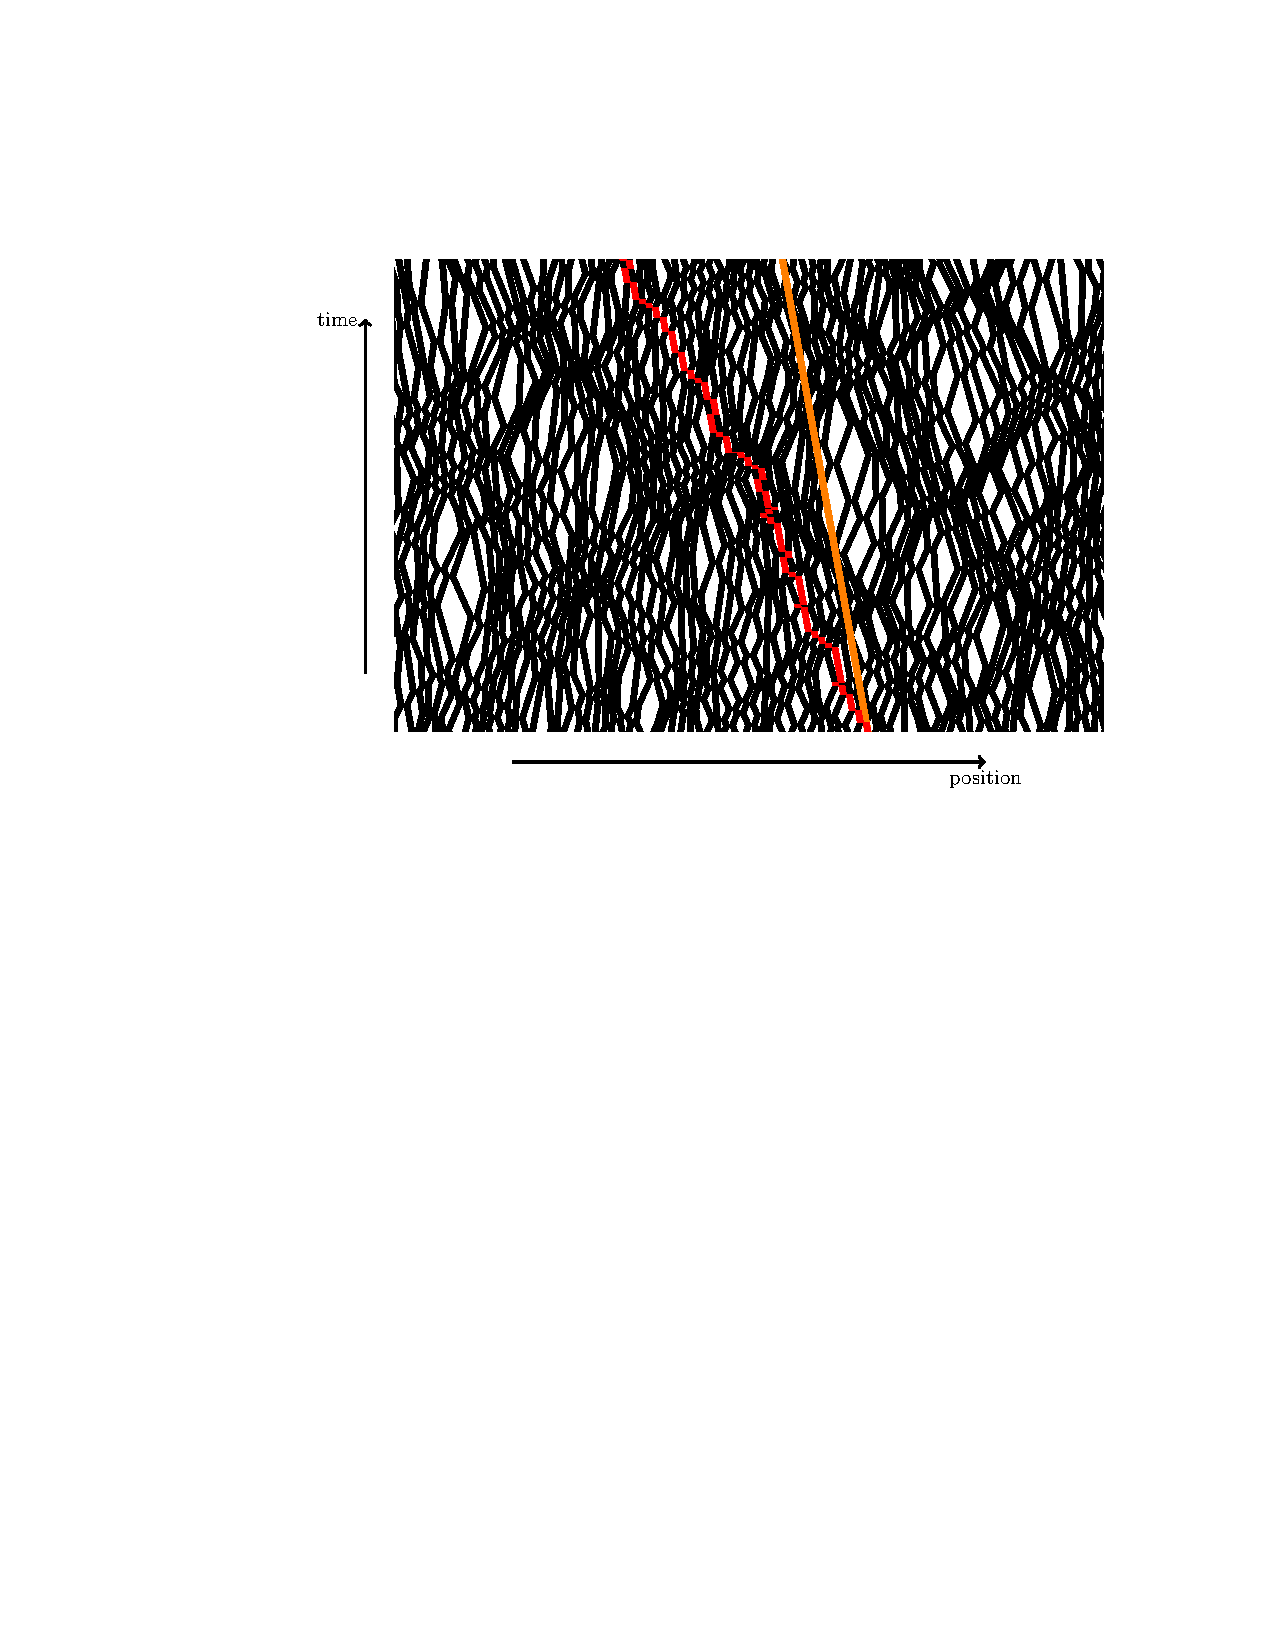
\includegraphics[width=0.6\textwidth]{doc/arXiv-2108.02509v2/figures/hardrods.pdf}};
    \end{tikzpicture}
    \caption{Le système le plus simple qui exhibe l'Hydrodynamique Généralisée' est sans doute le gaz de hard rod classique, c'est-à-dire des billes de billard identiques dont le mouvement est restreint à une ligne. À gauche : les billes entrent en collision de manière élastique et échangent leurs vitesses. On peut réindexer les billes après chaque collision de sorte que la vitesse 'nue' \(v_j\) soit constante (ici, la bille rouge est celle avec la vitesse \(v_2\) à tout moment). À droite : à des échelles de distance et de temps grandes, la vitesse effective de la bille rouge \(v^{\rm eff}\) (trajectoire rouge) est différente de sa vitesse 'nue' \(v\) (trajectoire orange). La description en termes d'Hydrodynamique Généralisée' du gaz de hard rod (\ref{eq:GHDintro}) est une limite hydrodynamique d'Euler où les interactions entre les particules entrent à travers la vitesse effective.}
    \label{fig:hardrod}
\end{figure}

On peut introduire une densité de phase espace grossière des billes \(\rho(x,v) = \sum_{j=1}^N \delta_\ell (x-x_j) \delta_\sigma (v-v_j)\), où \(\delta_\ell\) et \(\delta_\sigma\) sont des distributions lisses de poids un, concentrées autour de l'origine, par exemple deux Gaussiennes de largeur \(\ell\) et \(\sigma\). Lorsque \(\ell\) et \(\sigma\) sont suffisamment grands pour que le volume du phase space \([x,x+ \ell] \times [v,v+\sigma]\) contienne un très grand nombre de billes, mais assez petits pour que la densité reste constante à travers le volume, la densité grossière évolue selon les deux équations
\begin{equation}
    \label{eq:GHDintro}
    \left\{ \begin{array}{c}
       \displaystyle \partial_t \rho(x,v,t) + \partial_x \left( v^{\rm eff}[\rho](v) \, \rho(x,v,t) \right) - \frac{1}{m}\frac{\partial V(x)}{\partial x} \partial_v \rho(x,v,t) \, = \, 0, \\
       \displaystyle  v^{\rm eff}[\rho](v) = v - \Delta  \int_{-\infty}^\infty   \left( v^{\rm eff}[\rho](v) - v^{\rm eff}[\rho](w) \right)  \rho(w) dw ,
    \end{array} \right.
\end{equation}
où nous avons inclus un potentiel externe \(V(x)\). Ce sont les équations de l'Hydrodynamique Généralisée pour le gaz de hard rod, initialement dérivées par~\cite{percus1976equilibrium}, et prouvées par \cite{boldrighini1983one} pour \(V(x)=0\). L'inclusion du potentiel de piégeage, et sa rupture des lois de conservation, a été étudiée plus récemment par~\cite{cao2018incomplete}.

La première équation (\ref{eq:GHDintro}) est similaire à l'équation de transport (\ref{eq:liouville}), bien que deux différences importantes doivent être soulignées. La première différence réside dans le champ d'application de l'Eq.~(\ref{eq:GHDintro}) : il s'agit d'une description grossière du gaz de hard rod basée sur la relaxation locale, qui n'est valable qu'à l'échelle d'Euler. L'équation de transport libre~(\ref{eq:liouville}), en revanche, ne repose pas sur des hypothèses hydrodynamiques. La deuxième différence est qu'au lieu de la vitesse de groupe d'une seule particule, l'Eq.~(\ref{eq:GHDintro}) implique une 'vitesse effective'. Cette vitesse effective est une fonctionnelle de la densité \(\rho(v)\) à une position donnée \(x\) et un temps \(t\), définie par la deuxième équation (\ref{eq:GHDintro}). Elle a une interprétation simple, voir Fig.~\ref{fig:hardrod}. À chaque collision, les étiquettes des billes en collision peuvent être échangées, de sorte que chaque vitesse \(v_j\) reste constante, mais la position \(x_j\) change instantanément de \(\pm |\Delta|\) (le diamètre des billes). Pour une densité finie de billes, ces sauts entraînent une modification de la vitesse de propagation de la bille avec la vitesse \(v_j\) à travers le gaz, \(v_j \rightarrow v^{\rm eff}[\rho](v_j)\).

Les équations d'Hydrodynamique Généralisée~(\ref{eq:GHDintro}) sont également analogues aux équations hydrodynamiques d'Euler (\ref{eq:continuity3})-(\ref{eq:euler}), mais pour une infinité de charges. Toutes les charges sont conservées en l'absence de potentiel externe (\(V(x) = 0\)), tandis que pour \(V(x) \neq 0\), seule la conservation de la masse et de l'énergie est généralement attendue. Pour le voir, considérons les charges susmentionnées \(Q[f] = \sum_{j=1}^N f(v_j)\), et leurs densités de charge associées \(q[f](x,t) = \int_{-\infty}^\infty f(v) \rho(x,v,t) dv\). Ces densités de charge évoluent selon
\begin{equation}
    \label{eq:introGHD_continuity}
    \begin{array}{l}
   \displaystyle     \frac{\partial}{\partial t} q[f](x,t) + \frac{\partial}{\partial_x} j[f](x,t) \, = \, -\frac{1}{m} \frac{\partial V(x)}{\partial x} \int_{-\infty}^\infty  f'(v) \rho(x,v,t)  dv, \\
   \displaystyle {\rm avec}  \qquad j[f](x,t) = v^{\rm eff}[\rho](v) q[f](x,t) .
    \end{array}
\end{equation}
Lorsque \(V(x) = 0\), la première équation est une équation de continuité qui exprime la conservation de \(Q[f]\). La seconde ligne donne la valeur d'attente du courant en fonction des densités de charge sous les hypothèses hydrodynamiques.

Ainsi, comme affirmé ci-dessus, l'Hydrodynamique Généralisée capture un comportement particulier semblable à un fluide qui ressemble à la fois à un fluide obéissant à l'équation de transport libre~(\ref{eq:liouville}) et à un fluide obéissant aux équations hydrodynamiques d'Euler~(\ref{eq:continuity3},\ref{eq:euler}).

\vspace{0.5cm}

Remarquablement, les équations d'Hydrodynamique Généralisée (\ref{eq:GHDintro}) ont réémergé en 2016, dans le contexte des systèmes quantiques intégrables unidimensionnels~\citep{castro2016emergent,bertini2016transport}. Dans la décennie qui a précédé cette percée de 2016, d'énormes progrès avaient été réalisés sur la dynamique quantique hors d'équilibre, largement motivés par les avancées dans les expériences sur les atomes froids. Pour ne citer qu'un exemple, l'expérience de 2006 du Quantum Newton Cradle de~\cite{kinoshita2006quantum}, où deux nuages unidimensionnels d'atomes interagissants dans un potentiel harmonique \(V(x)\) subissent des milliers de collisions, échappant apparemment à la convergence vers l'équilibre thermique, était devenue une source d'inspiration importante et un défi pour les théoriciens des systèmes quantiques à plusieurs corps. De nombreuses avancées conceptuelles importantes sur la thermalisation (ou son absence) des systèmes quantiques isolés, en particulier les développements autour de la notion d'Ensemble de Gibbs généralisé, ont eu lieu entre 2006 et 2016. Pourtant, une modélisation quantitativement fiable de la configuration du Quantum Newton Cradle, avec des paramètres expérimentalement réalistes, était restée complètement hors de portée. Comme d'habitude avec les systèmes quantiques à plusieurs corps, la croissance exponentielle de l'espace de Hilbert avec le nombre d'atomes \(N\) empêchait apparemment des simulations numériques directes de la dynamique.

La percée de 2016 de l'Hydrodynamique Généralisée a complètement changé cet état de choses. La réalisation que la dynamique des gaz quantiques ultrafroids unidimensionnels dans des expériences telles que le Quantum Newton Cradle est capturée par des équations d'Hydrodynamique Généralisée de la forme (\ref{eq:GHDintro}) a ouvert une nouvelle ère pour leur description théorique.

\vspace{1cm}

{\bf Objectif de cette revue et organisation.} Notre but est de 
fournir un aperçu pédagogique des développements qui ont eu lieu sur le gaz de Bose unidimensionnel depuis la découverte en 2016 de l'Hydrodynamique Généralisée dans les systèmes quantiques intégrables \citep{castro2016emergent,bertini2016transport}. Étant donné que le sujet intéresse à la fois les physiciens des atomes froids et les physiciens statistiques quantiques, nous avons tenté d'écrire cet article de revue de manière à le rendre accessible à tous.

L'article est organisé comme suit. Dans la section~\ref{sec:LiebLiniger}, nous examinons les faits de base concernant la théorie du gaz de Bose unidimensionnel qui sont utiles pour comprendre le développement de l'Hydrodynamique Généralisée. Nous fournissons une introduction au modèle de Lieb-Liniger répulsif, en mettant fortement l'accent sur le concept clé des rapidités. Nous passons également en revue les régimes asymptotiques du gaz de Bose unidimensionnel (quasicondensat, gaz de Bose idéal et régimes à cœur dur), qui sont souvent importants dans la description des expériences. Dans la section~\ref{sec:GHDtheory}, nous présentons la description de l'Hydrodynamique Généralisée du gaz de Bose unidimensionnel et passons en revue les résultats théoriques qui ont été obtenus depuis 2016 avec cette approche. Dans la section~\ref{sec:experiments_beforeGHD}, nous passons brièvement en revue les configurations expérimentales qui ont été utilisées pour réaliser des gaz de Bose unidimensionnels, ainsi que les principaux résultats expérimentaux obtenus en lien avec l'intégrabilité. Dans cette section, nous nous concentrons principalement sur les résultats obtenus avant l'avènement de l'Hydrodynamique Généralisée. Ensuite, dans la section~\ref{sec:GHDexperiment}, nous présentons les tests expérimentaux de l'Hydrodynamique Généralisée et les expériences récentes dont les descriptions ont reposé sur l'Hydrodynamique Généralisée. Dans la section~\ref{sec:losses}, nous discutons brièvement des récents développements théoriques visant à décrire l'effet des pertes d'atomes. Nous discutons de certaines perspectives et questions ouvertes dans la Conclusion.


 
 
 
 